\documentclass[defaultstyle,10pt,master,Helvetica]{01.thesis}

\usepackage[T1]{fontenc}
\usepackage{titlesec, blindtext, color}
%% Packages
\typeout{}
\typeout{--------------------------------------------------------------}
\typeout{ +---+ Thesis Template                            }
\typeout{ +---+      Version 2.0, August 2011                         }
\typeout{ +---+  for Instituto Superior Tecnico (IST),                 }
\typeout{ +---+  Universidade Técnica de Lisboa                         }
\typeout{ * Using Thesis Style from Pedro Tomás                                }
\typeout{ * Created to write Dissertations                             }
\typeout{ * Conforms with IST Master Degree format and with most important packages setup        }
\typeout{ * Should conform with IST PhD Degree format (not verified)   }
\typeout{                                                              }
\typeout{ AUTHOR: Miguel Amador and João Marques                                          }
\typeout{                                                              }
\typeout{Important: Use all files in the archive, since this is based in all them. Modify dummy files at wish.                                                              }
\typeout{--------------------------------------------------------------}
\typeout{}

% Defines an additional alphabet... not required in most cases
% ------------------------------------------------------------
% \DeclareMathAlphabet{\mathpzc}{OT1}{pzc}{m}{it}

% PACKAGE babel:
% ---------------
% The 'babel' package may correct some hyphenisation issues of latex. 
% However in most situations it is not required.
\usepackage[english,portuguese]{babel}


% PACKAGE fontenc:
% -----------------
% chooses T1-fonts and allows correct automatic hyphenation.
%\usepackage[T1]{fontenc}
%\usepackage[latin1]{inputenc}
\usepackage[utf8]{inputenc}
%\usepackage{lmodern}

% Package ulem.
\usepackage{ulem} % Allows the use of other text emphatizer commands
\normalem %defines \emph{} to italic, instead of underline. 
\raggedbottom %declaration makes all pages the height of the text on that page. No extra vertical space is added. The \flushbottom declaration makes all text pages the same height, adding extra vertical space when necessary to fill out the page.

% PACKAGE date time:
% -----------------
% Lets you alter the format of the date that \today returns.
\usepackage{datetime}
\newdateformat{todaythesis}{%
\monthname[\THEMONTH]  \THEYEAR}

% PACKAGE latexsym:
% -----------------
% Defines additional latex symbols. May be required for thesis with many math symbols.
\usepackage{latexsym}

% PACKAGE amsmath, amsthm, amssymb, amsfonts:
% -------------------------------------------
% This package is typically required. Among many other things it adds the possibility
% to put symbols in bold by using \boldsymbol (not \mathbf); defines additional 
% fonts and symbols; adds the \eqref command for citing equations. I prefer the style
% "(x.xx)" for referering to an equation than to use "equation x.xx".
\usepackage{amsmath, amsthm, amssymb, amsfonts, amsbsy}

% PACKAGE multirow, colortbl, longtable:
% ---------------------------------------
% These packages are most usefull for advanced tables. The first allows to join rows 
% throuhg the command \multirow which works similarly with the command \multicolumn
% The second package allows to color the table (both foreground and background)
% The third package is only required when tables extend beyond the length of one page;
% with compatibilities with the tabular environment. The last allow the definitions of landscape pages, allowing the use of a different orientation for wider graphics or tables. See package documentation to see the implementation.
\usepackage{multirow}
\usepackage{colortbl}
\usepackage{supertabular}
\usepackage{pdflscape}
% \usepackage{longtable}

% PACKAGE graphics, epsfig, subfigure, caption:
% ---------------------------------------------
% Packages for figures... well you will certainly need these packages, with the exception
% of the 'caption' package. This only allows to define extra caption options.
% Notice that subfigure allows to place figures within figures with its own caption. It
% should be avoided to create an eps file with subfigures. That will mean that you won't be 
% able to reference those subfigures. Instead create an EPS file (the only graphics format supported
% by latex) for each of the subfigures and then use the command \subfigure (see below).
\usepackage{graphics}
\usepackage{graphicx}
\usepackage{epsfig}
\usepackage[hang,small,bf]{subfigure}
%\usepackage[footnotesize,bf,center]{caption}
\usepackage{dcolumn}
\usepackage{bm}
\usepackage{booktabs}
\usepackage{rotating}
\usepackage{multirow}

\usepackage[font=small,labelfont=bf,textfont=normalfont]{caption}

% PACKAGE algorithmic, algorithm
% ------------------------------
% These packages are required if you need to describe an algorithm.
% \usepackage{algorithmic}
% \usepackage[chapter]{algorithm}

% PACKAGE natbib/cite
% -------------------
% The two packages are not compatible, and you should use one of the two. Notice however that the
% IEEE BiBTeX stylesheet is imcompatible with the natbib package. If using the IEEE format, use the 
% cite package instead
\usepackage[square,numbers,sort&compress]{natbib}
%\usepackage{cite}

% PACKAGE acronyum
% -----------------
% This package is most useful for acronyms. The package guarantees that all acronyms definitions are 
% given at the first usage. IMPORTANT: do not use acronyms in titles/captions; otherwise the definition 
% will appear on the table of contents.
\usepackage[printonlyused]{acronym}
\usepackage[titletoc,title,header]{appendix}
\usepackage[noauto]{chappg}

% PACKAGE extra_functions VER COMO DEVE SER
% -----------------
% My Personal package: defines the following commands:
% \fancychapter{chaptername) -> Prints a fancier chapter (you can also use the fancychapter package for this)
% \hline{width} -> use for a replacement of the \hline command
% \Mark1, \Mark2, \Mark3, ...
\usepackage{00.extra_functions}


% PACKAGE hyperref
% -----------------
% Set links for references and citations in document
% Some MiKTeX distributions have faulty PDF creators in which case this package will not work correctly
% Long live Linux :D
\usepackage[plainpages=false]{hyperref}
\hypersetup{
             colorlinks=false,
             citecolor=red,
             breaklinks=true,
             bookmarksnumbered=true,
             bookmarksopen=true,
             pdftitle={Thesis Title},
             pdfauthor={Author Name},
             pdfsubject={Master Thesis in Biomedical Engineering},
             pdfcreator={Document Creator Name},
             pdfkeywords={Template, Latex, Thesis}}
\usepackage{float}
%\usepackage[final]{00.listofsymbols}
\usepackage{00.symlist}

% Set paragraph counter to alphanumeric mode
\renewcommand{\theparagraph}{\Alph{paragraph}~--}

\newcommand{\figref}[1]{Figure \ref{#1}}
\newcommand{\equationref}[1]{Equation (\ref{#1})}
\newcommand{\tableref}[1]{Table (\ref{#1})}

\newcommand{\textreg}{$\textsuperscript{\textregistered}$}
%% Page formatting
\hoffset 0in
\voffset 0in

%Alternative set of page geometry
%\oddsidemargin 0.71cm
%\evensidemargin 0.04cm
%\marginparsep 0in
%\topmargin -0.25cm
%\textwidth 15cm
%\textheight 23.5cm

\usepackage[top=2.5cm, bottom=2.5cm, inner=2.9cm, outer=2.5cm]{geometry}

\usepackage{fancyhdr}
\pagestyle{fancy}
\renewcommand{\chaptermark}[1]{\markboth{\thechapter.\ #1}{}}
\renewcommand{\sectionmark}[1]{\markright{\thesection\ #1}}
\fancyhf{} 
%\fancyhead[LE]{\bfseries\nouppercase{\leftmark}}
%\fancyhead[RO]{\bfseries\nouppercase{\rightmark}}
\fancyfoot[LE,RO]{\bfseries\small\thepage}
\renewcommand{\headrulewidth}{0.0pt}
\renewcommand{\footrulewidth}{0.0pt}
\addtolength{\headheight}{2pt} % make space for the rule
\fancypagestyle{plain}{% Used in Chapter titles
   \fancyhead{} % get rid of headers
   \renewcommand{\headrulewidth}{0pt} % and the line
   \renewcommand{\footrulewidth}{0pt}
   \fancyfoot[LE,RO]{\bfseries\small\thepage}
}

\fancypagestyle{begin}{%
   \fancyhead{}
   \renewcommand{\headrulewidth}{0pt}
   \renewcommand{\footrulewidth}{0pt}
   \fancyfoot[LE,RO]{\bfseries\small\thepage}
}
\fancypagestyle{document}{%
	\fancyhf{} 
	\fancyhead[LE]{\bfseries\nouppercase{\leftmark}}
	\fancyhead[RO]{\bfseries\nouppercase{\rightmark}}
	\fancyfoot[LE,RO]{\bfseries\small\thepage}
	%\renewcommand{\headrulewidth}{0pt}
	%\renewcommand{\footrulewidth}{0pt}
	\addtolength{\headheight}{2pt} % make space for the rule
}
\fancypagestyle{documentsimple}{%
	\fancyhf{}
	\fancyfoot[LE,RO]{\bfseries\small\thepage}
	%\renewcommand{\headrulewidth}{0pt}
	%\renewcommand{\footrulewidth}{0pt}
	\addtolength{\headheight}{2pt} % make space for the rule
}
\setcounter{secnumdepth} {5}
\setcounter{tocdepth} {5}
\renewcommand{\thesubsubsection}{\thesubsection.\Alph{subsubsection}}

\renewcommand{\subfigtopskip}{0.3 cm}
\renewcommand{\subfigbottomskip}{0.2 cm}
\renewcommand{\subfigcapskip}{0.3 cm}
\renewcommand{\subfigcapmargin}{0.2 cm}

\graphicspath{{Figures/}}

%% NEW CHAPTER STYLE %%%
\usepackage[T1]{fontenc}
\usepackage{titlesec, blindtext, color}
\definecolor{gray75}{gray}{0.75}
\newcommand{\hsp}{\hspace{20pt}}
\titleformat{\chapter}[hang]{\Huge\bfseries}{\thechapter\hsp\textcolor{gray75}{|}\hsp}{0pt}{\Huge\bfseries}


%-----------------------------------------------------------
%-----------------------------------------------------------
\begin{document}
%% Use Main document Language
\selectlanguage{english}
%% ------
\pagestyle{begin}
\setcounter{page}{1} \pagenumbering{Alph}

% Add PDF bookmark 
\pdfbookmark[0]{Title}{Title}

\thispagestyle{empty}
\begin{flushleft} ~\\ \vspace{-12mm} \hspace{-12mm}  \includegraphics[width=50mm]{Cover/istnewlogo} 
\vspace{10mm}
%~\\ \vspace{50mm} % gráficos
\\ \begin{center} 
\includegraphics[width=1\linewidth]{Cover/coverimage}  \end{center} % gráficos
 \vspace{5mm}
\centering
\LARGE \textbf{Thermographical analysis of interface heat transfer mechanisms, with high time precision}
%\\ \vspace{10mm}
%\Large Subtitle
\\ \vspace{15mm}
\Large \textbf{Pedro Daniel Fernandes Pontes} \\
\vspace{12mm}
\large Thesis to obtain the Master of Science Degree in
\\ \vspace{2mm}
\LARGE \textbf{Mechanical Engineering}
\\ \vspace{10mm}
\large Supervisor(s): Prof./Dr. Ana Sofia Oliveira Henriques Moita 
\\ \vspace{15mm}
\Large \textbf{Examination Committee}
\\ \vspace{5mm}
\large Chairperson:	Prof. Lorem \\
\large Supervisor: Prof. Lorem Ipsum\\
\large Co-Supervisor: Prof. Lorem Ipsum \\
\large Members of the Committe: Dr. Lorem Ipsum \\
Prof. Lorem Ipsum
 
\vspace{15mm}

%\Large \textbf{\todaythesis\today} \\
\Large \textbf{October 2016} \\
\let\thepage\relax
\end{flushleft}
\pagebreak


\clearpage
% Since I am using double sided pages, the second page should be white.
% Remember that when delivering the dissertation, IST requires for the cover to appear twice.

\thispagestyle{empty}
\cleardoublepage

\setcounter{page}{1} \pagenumbering{roman}

\baselineskip 18pt % line spacing: -12pt for single spacing
                   %               -18pt for 1 1/2 spacing
                   %               -24pt for double spacingnts} 
\thispagestyle{empty}
\pdfbookmark{Acknowledgments}{Acknowledgments}

\begin{acknowledgments} 

%First would like to thank IST for being my home and teaching me everything I needed to get this far. It has been truly amazing studying here and knowing so many inspiring teachers and so many brilliant colleagues.
\par - prof e ema
\par - co-workers
\par - friends
\par - family and fu
\par - outros?


\end{acknowledgments}

\hbox{} \vfill
\begin{flushright}
\small \textit{\textbf{"Try not to become a person of success, but rather try to become a person of value."}} %%% MUDAR %%%
\\ \vspace{2mm}  
\scriptsize Albert Einstein
\end{flushright}

\clearpage
\thispagestyle{empty}
\cleardoublepage
%\pdfbookmark{Acknowledgments}{Acknowledgments}
\begin{acknowledgments} 

I would like to thank the Academy, bla bla bla..

\end{acknowledgments}
\clearpage
\thispagestyle{empty}
\cleardoublepage
\selectlanguage{english}
\begin{abstract}

bla bla

\end{abstract}
\begin{keywords}
Keywords (English)
\end{keywords}
\clearpage
\thispagestyle{empty}
\cleardoublepage
\selectlanguage{portuguese}
\begin{resumo}

O objectivo deste trabalho ... (Português)

\end{resumo}
\begin{palavraschave}
Palavras-Chave (Português)
\end{palavraschave}
\clearpage
\thispagestyle{empty}
\cleardoublepage
%% Use Main document Language
\selectlanguage{english}
%% ------
% This is required for the fancy chapters
\dominitoc
\dominilof
\dominilot

%%%%%%%%%%%%%%%%%%%%%%%%%%%%%%%%%%%%%%%%%%%%%%%%%%%%%%%%%%%%%%%%%%%%%%
% List of contents
%\renewcommand{\baselinestretch}{1}
\pdfbookmark[0]{Index}{index}
\pdfbookmark[1]{Contents}{toc}
\tableofcontents
% \contentsline{chapter}{References}{\pageref{bib}}
\clearpage
\thispagestyle{empty}
\cleardoublepage
%\renewcommand{\baselinestretch}{1.5}
%%%%%%%%%%%%%%%%%%%%%%%%%%%%%%%%%%%%%%%%%%%%%%%%%%%%%%%%%%%%%%%%%%%%%%
% List of figures
\pdfbookmark[1]{List of Figures}{lof}
\listoffigures
\clearpage
\thispagestyle{empty}
\cleardoublepage

%%%%%%%%%%%%%%%%%%%%%%%%%%%%%%%%%%%%%%%%%%%%%%%%%%%%%%%%%%%%%%%%%%%%%%
% List of tables
\pdfbookmark[1]{List of Tables}{lot}
\listoftables
\clearpage
\thispagestyle{empty}
\cleardoublepage

% %%%%%%%%%%%%%%%%%%%%%%%%%%%%%%%%%%%%%%%%%%%%%%%%%%%%%%%%%%%%%%%%%%%%%%
% % List of algorithms
% Requires packages algorithmic, algorithm
% \pdfbookmark[1]{List of Algorithms}{loa}
% \listofalgorithms
% \cleardoublepage
\acresetall
%% Remain list of table titles are set manualy
% %%%%%%%%%%%%%%%%%%%%%%%%%%%%%%%%%%%%%%%%%%%%%%%%%%%%%%%%%%%%%%%%%%%%%%
 % List of acronyms
\pdfbookmark[1]{List of Acronyms}{loac}

\chapter*{Abbreviations}


% See more at http://staff.science.uva.nl/~polko/HOWTO/LATEX/acronym.html

\begin{acronym}
\acro{acro}{Dummy Acronym}
\end{acronym}

\clearpage
\thispagestyle{empty}
\cleardoublepage




%%%%%%%%%%%%%%%%%%%%%%%%%%%%%%%%%%%%%%%%%%%%%%%%%%%%%%%%%%%%%%%%%%%%%%
% List of symbols
\pdfbookmark[1]{List of Symbols}{los}

\listofsymbols

\clearpage
\thispagestyle{empty}

\cleardoublepage
% Pages number is starting now with arabic style... until now it was on roman mode
\pagenumbering{arabic} \setcounter{page}{1}
\baselineskip 18pt
%% Use Main document Language
\selectlanguage{english}
%% Define the title of Chapter Table of Contents
\mtcsettitle{minitoc}{Contents}
%% ------
\pagestyle{documentsimple}%Simple head
% %%%%%%%%%%%%%%%%%%%%%%%%%%%%%%%%%%%%%%%%%%%%%%%%%%%%%%%%%%%%%%%%%%%%%%
% The Introduction:
% %%%%%%%%%%%%%%%%%%%%%%%%%%%%%%%%%%%%%%%%%%%%%%%%%%%%%%%%%%%%%%%%%%%%%%
\chapter{Introduction}
\label{cap:int}

\section{Motivation}
\label{sec:int_motivation}

\par Heat transfer in fluid-solid interfaces, with fluid state change, is a common phenomena in the nature and technology. It is still a mystery, although getting smaller with time, what mechanisms transfer heat during boiling. Because there are countless applications in the industry where this phenomena occurs, there is a need to know what actually is happening so we can then improve these applications by more efficiently controlling them. \\
\par Surface heat removal using liquids is a complex and fast happening that often involves state change. So, to study this type of phenomena, we need high precision equipment with, not only high spatial precision, but also time precision. In this field of study, many types of measuring equipment have been used to quantify and qualify such phenomena. The use of a thermocouple, for instance, which is a really common method, can be intrusive to the measured process, can only measure one point and cannot be in contact with electricity. With this in mind, infra-red thermography has been a great alternative to some of the existing intrusive temperature measuring methods. A thermographical camera with a good calibration can give high precision temperature results at high frame rates, which can give high definition qualitatively and, more importantly, quantitatively accurate thermal images. The IR camera also outputs two dimensional images, a great advantage when trying to understand this kinds of processes. \\
\par Although the IR camera use will be centered in the boiling process, the heat transfer mechanisms in droplet surface impact will also be studied. Both require high precision results, so calibration and result processing should be studied with great care. \\
\par While this work is developed, a computational study by Emanuele Teodori is being made, and this work's results will also be used to validate the computational model in use.
\section{State of The Art}
\label{sec:int_state}

State of The Art Section.

\subsection{Dummy Subsection A}
\label{subsec:subsectiona}

State of Art Subsection A

\subsection{Dummy Subsection B}
\label{subsec:subsectionb}

State of Art Subsection B


\section{Objectives}
\label{sec:int_contributions}

\par The main objective of this dissertation is to optimize the use of the IR Camera to study interface phenomena in droplet impact. This not only includes improving studying the positioning of the camera and data processing, but also study the techniques that are involved in getting to the heat transfer in the various interfaces. The techniques used will be an adaptation of what previous authors did using thin foil surfaces, always trying to improve both the time and spatial resolution.\\

\par To achieve good quantitative results with the camera, it is of the most importance that this camera is properly calibrated, so another important objective will be create a process that can accurately calibrate a camera for the laboratory's use. To add to a good calibration it will be also very important to create quality IR data processing tools that can be used in future work.\\

\par One last objective will be to vary the experiments variables and analyze if the collected images react as expected to the variation. This setup will be tested with foils at under, during and over saturation temperature, with an elevated and lower droplet impact velocity, with different liquids and also different surface wettability. This will evaluate if the improvements to the existent method allowed better results.
\section{Thesis Outline}
\label{sec:int_outline}

\par In this work an introduction to the used concepts will be given. This will go through IR thermography, wettability and droplet impact physics and heat transfer phenomena. This introduction will be presented in Chapter 2.\\

\par In Chapter 3, the 2 conceived experimental setups will be explained. This will include explanation about the role of every material present in the setup and also the process of collecting data. The functioning of the IR Camera will be clarified aswell as the data collecting methods and software calibration options.\\

\par One of the most important parts of this work is the proposed calibration. In Chapter 4, the proposed calibration method will be explained and compared against the existing calibration. All the thought process behind the calibration and its construction will be shown. The data processing code that was made specially for this camera is also explained in this chapter and its effects shown.\\

\par The results of the experiments in various conditions will be presented in Chapter 5, along with the observed phenomena, making a bridge between the expected results, from the introductory chapter, and the obtained ones. The conclusions about these results and the used method will be discussed in Chapter 6 and clarified if the proposed objectives were reached. Also in this chapter, future work that will be developed around this method will be discussed.

\cleardoublepage
% %%%%%%%%%%%%%%%%%%%%%%%%%%%%%%%%%%%%%%%%%%%%%%%%%%%%%%%%%%%%%%%%%%%%%%
% Dummy Chapter:
% %%%%%%%%%%%%%%%%%%%%%%%%%%%%%%%%%%%%%%%%%%%%%%%%%%%%%%%%%%%%%%%%%%%%%%

% %%%%%%%%%%%%%%%%%%%%%%%%%%%%%%%%%%%%%%%%%%%%%%%%%%%%%%%%%%%%%%%%%%%%%%
% The Introduction:
% %%%%%%%%%%%%%%%%%%%%%%%%%%%%%%%%%%%%%%%%%%%%%%%%%%%%%%%%%%%%%%%%%%%%%%
\chapter{Theoretical Background}
\label{cap:theoretical}

\textit{In this chapter some theoretical background will be given about what's going to be discussed further.}

\section{Infrared Thermography}
\label{sec:sectiona}

Heat transfer through radiation is the way, in thermography, most often used to gather it's results and one of the main objects of study of this work is how to correctly transform the measured radiation intensity plus the information on the body emissivity and surrounding conditions in an accurate temperature estimate. To do so, some theoretical notions will have to be mentioned so that thermography can be better understood.

\subsection{Radiation Intensity to Temperature Conversion}
\label{subsec:rad2tem}

Radiation is emitted by all bodies at $T>0$. The intensity of this radiation largely depends on the direction, wavelength and of course temperatures. For example, above 500ºC, a body's radiation is almost entirely in the IR wavelength \cite{IRCAM}. Besides emitting radiation a body can also absorb ($\alpha$), reflect ($\rho$) and radiation can even pass through it ($\tau$). Adding all this elements we get the Total Radiation Law:
\begin{equation}
    W = W\alpha + W\rho + W\tau
\end{equation}
... in which $W$ represents the total energy transmitted through radiation. Using a simplified version we can also say that:
\begin{equation}\label{eq:1}
	1 = \alpha + \rho + \tau
\end{equation}
Note that in the equation \ref{eq:1}, $\alpha$, $\rho$ and $\tau$ represent their respective fractions of the incident radiation energy, and need to have values between 0 and 1.\\

\subsubsection{Blackbody Equations}

\par One of the most important concepts that is used in this work is the concept of \textit{blackbody}. A \textit{blackbody} is characterized for absorbing all energy transmitted through radiation. In the ideal case of a \textit{blackbody} the coefficients assume the following values: $\alpha=1, \ \rho=0, \ \tau=0$. The blackbody is also a perfect emitter. The emissivity ($\varepsilon$) of a body characterizes the efficiency of a body for emitting energy, so it's the ratio between energy emitted and the energy emitted if the body was a \textit{blackbody}. With this in mind we can use the equation \ref{eq:2} for a \textit{blackbody}. This equation is called Kirchhoff Law. Kirchhoff Law is also applied for the same wavelength ($\lambda$) so we can also use equation \ref{eq:3}.

\begin{equation}\label{eq:2}
\alpha=\varepsilon
\end{equation}
\begin{equation}\label{eq:3}
\alpha(\lambda)=\varepsilon(\lambda)
\end{equation}
\par For the specific case of a \textit{blackbody} we can also apply equation \ref{eq:4}. This equation is called Stefan-Boltzmann law and it states the relation between energy emitted through radiation and the temperature of the body. If the body is not perfectly black, but it's absorption/reflection/transparency properties don't vary with the wavelength, we call it a \textit{greybody} and can use equation \ref{eq:5}.
\begin{equation}\label{eq:4}
W=\sigma T^4
\end{equation}
\begin{equation}\label{eq:5}
W=\varepsilon \sigma T^4
\end{equation}
...where $\sigma=5.670373 \times 10^8 W m^{-2} K^{-4}$ and it's called the Stefan-Boltzmann constant.\\
\par It's fairly obvious these are concepts that illustrate ideal situations, and even though in most experiments shown further ahead the materials are chosen to be as close to \textit{black} or \textit{greybodies}, those aren't perfect. Of course this is attenuated by the fact that thermography measures in small intervals of wavelength. The next subsection will relate how does one choose a wavelength interval, and it's relation with the atmosphere.

\subsubsection{Atmosphere Attenuation}
\label{subsec:atmat}

\par The thing that separates almost every thermographical camera from its target is the atmosphere, which has good and bad transmittance in different wavelengths. The atmosphere attenuation comes with the complexity of it's composition. For example, each of the following molecules: $H_2O$, $O_2$, $CO_2$ have certain wavelength values for which $\tau=0$. This means that in these wavelengths IR radiation will not pass through the atmosphere and its intensity cannot be measured.\\
\par This issue calls for the necessity of choosing a wavelength \textit{window} for which the transmittance is close to 1. These \textit{windows} can be seen in Figure \ref{fig:atm}. It is possible to identify 2 main regions: the medium-wave \textit{window} (from 2-5 $m \mu$), or MW, and the long-wave \textit{window} (from 7.5-13.5 $m \mu$), or LW. The used camera works in the MW range so a selective range of wavelength inside it had to be chosen so to avoid bad atmosphere transmittance.

\begin{figure}
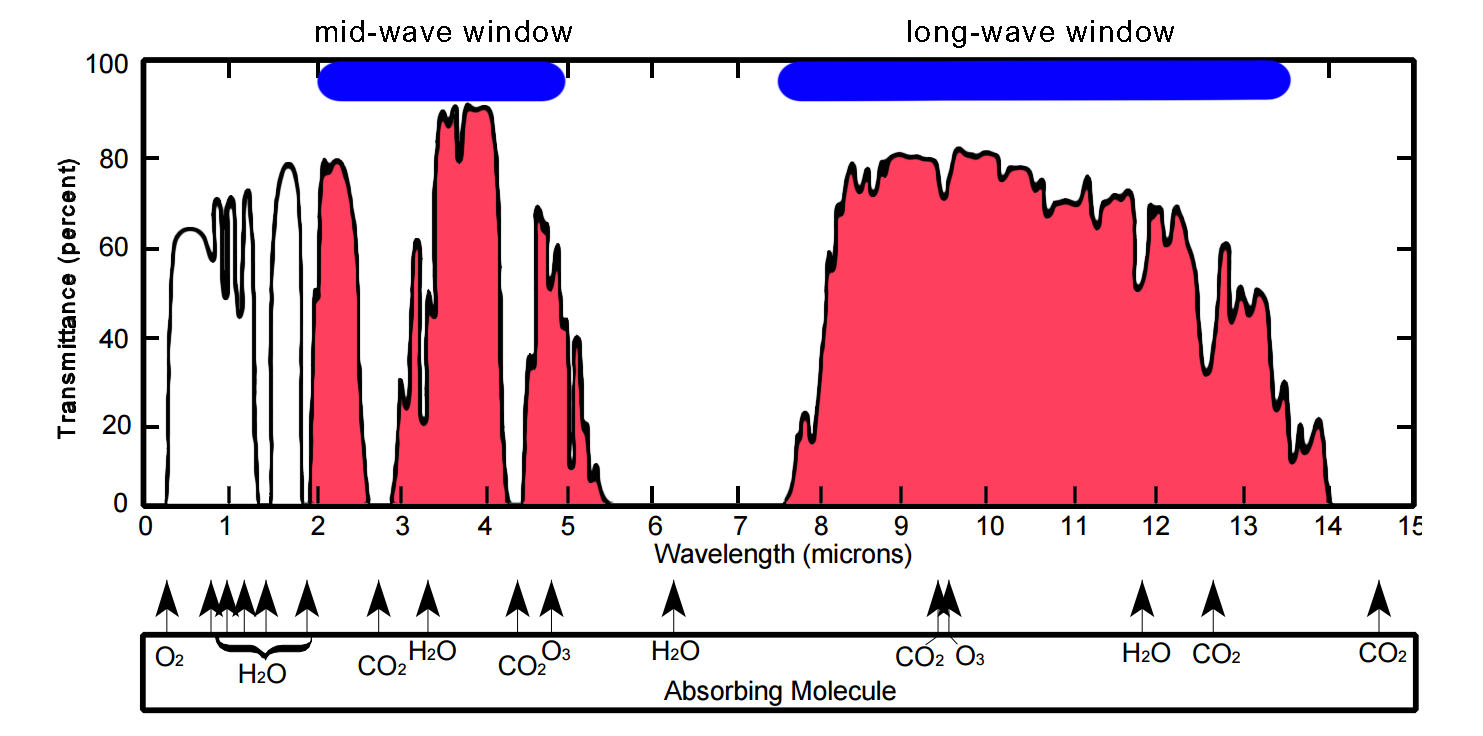
\includegraphics[width=1\linewidth]{Figures/2.Chapter/atmospheric_window.png}
\caption{Atmospheric Windows}
\source{Adaptation from chapter 7's Figure 10 of \cite{desk1997electronic}}
\label{fig:atm}
\end{figure}

\subsubsection{Total Radiation}
\par When measuring a body's temperature with the IR Camera, there are other radiation sources that have to be accounted for. In total we can divide these radiation sources in 3 categories, shown bellow wi:
\begin{itemize}
\item The radiation emitted by the object/objects of study
\begin{equation}
W_{obj}=\varepsilon_{obj} \ \sigma \ T_{obj}^4
\end{equation}
\item The radiation emitted by the atmosphere (where $ \ \varepsilon_{atm}=1-\tau_{atm}$ because $\rho_{atm}~=0$)
\begin{equation}
W_{atm}= (1-\tau_{atm}) \ \sigma \ T_{atm}^4
\end{equation}
\item The radiation from the surroundings reflected by the object/objects.
\end{itemize}
\begin{equation}
W_{refl}=(1-\varepsilon_{obj}) \ \sigma \ T_{refl}^4
\end{equation}
...where $T_{refl}$ refers to the apparent temperature of the surrounding that's radiating to the body.\\
\par Figure \ref{fig:camscheme} describes these sources and their origin. Note all the expressions in the figure represent energy radiated. In it it's possible to observe 2 sources of radiation come from the studied body represent the emitted and reflected components. When these components cross the atmosphere, they're affected by its transmissivity, $\tau_{atm}$ (this value in common atmospheric conditions is close to 1). The atmosphere itself can emit radiation, but because $\tau_{atm}$ is so close to 1, it mostly negligible.\\

\begin{figure}
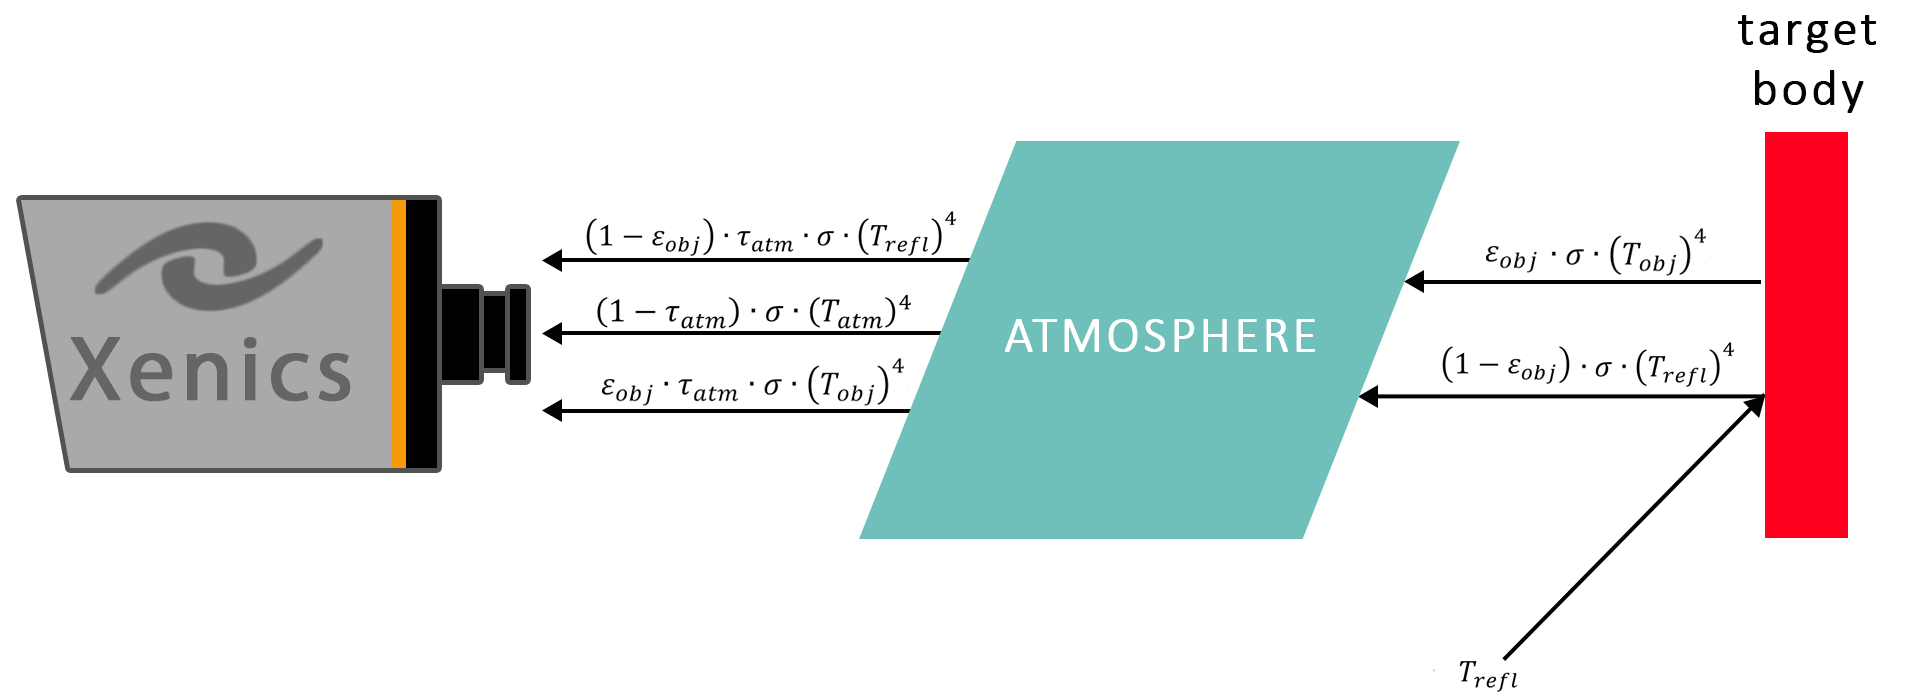
\includegraphics[width=1\linewidth]{Figures/2.Chapter/ir_camera_radiation_scheme.png}
\caption{Total radiation sources scheme}
\label{fig:camscheme}
\end{figure}

\par With these equations it is possible to relate the radiated energy received $W$ and the body temperature. This relation is demonstrated in equation \ref{eq:6} and \ref{eq:7}.
\begin{equation}\label{eq:6}
W_{tot}=W_{obj}+W_{refl}+W_{atm}=(\varepsilon_{obj} \ \sigma \ T_{obj}^4)+((1-\varepsilon_{obj}) \ \sigma \ T_{refl}^4)+((1-\tau_{atm}) \ \sigma \ T_{atm}^4)
\end{equation}
\begin{equation}\label{eq:7}
T_{obj}=\sqrt[4]{\frac{W_{tot}-(1-\varepsilon_{obj}) \ \sigma \ T_{refl}^4-(1-\tau_{atm}) \ \sigma \ T_{atm}^4}{\sigma \ \varepsilon_{obj}}}
\end{equation}
\par The camera receives the total radiation $W_{tot}$, and the user has to input the emissivity and both the ambient and reflection temperatures in the camera software.

\section{Wettability}

\par Wettability is a qualitative surface property that describes how the surface is wetted by a liquid. This property is characterized by the interface tensions between the present solid, liquid and gaseous states. The balance between these tensions is represented in Figure \ref{fig:tensao}
\begin{figure}[h]
\centering
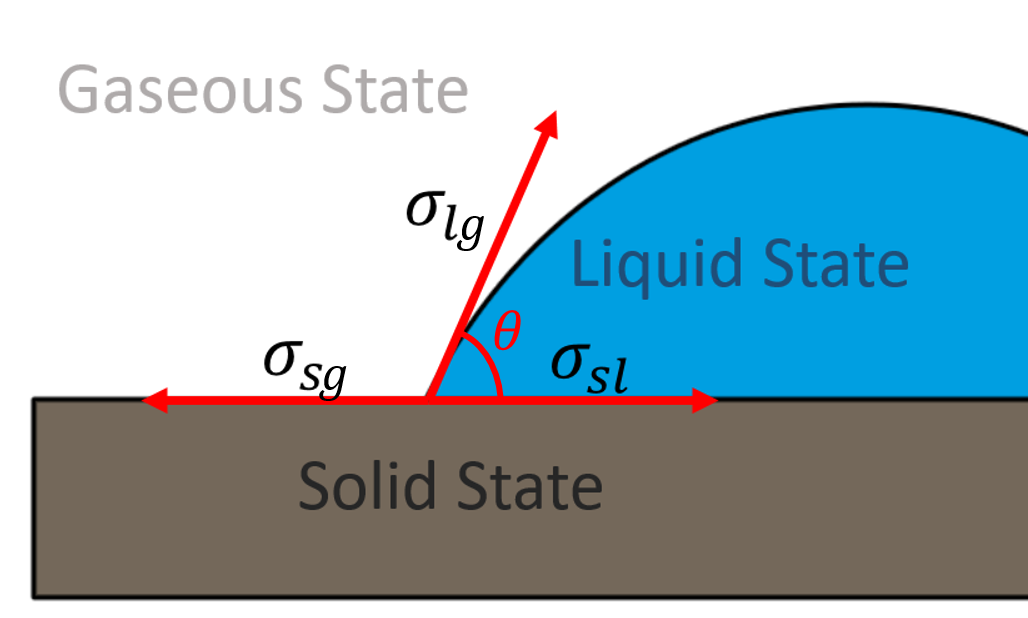
\includegraphics[width=0.5\linewidth]{Figures/2.Chapter/tensao.PNG}
\caption{Tension Balance}
\label{fig:tensao}
\end{figure}
\par Wettability has several parameters that characterize it, being the most used one the contact angle of a sessile droplet onto a flat rigid face. In a thermodynamics perspective, the equilibrium condition of a liquid droplet are calculated by the minimization of the Gibbs energy of the system, G. When one considers constant temperature and pressure conditions it is possible to write the famous Young's equation \cite{young1805essay} from this minimization ($dG=0$), which is simply the tension balance in the horizontal axis:
\begin{equation}
\sigma_{sg}=\sigma_{sl}+\sigma_{lg}cos(\theta_e)
\end{equation}
where $\sigma$ represents the interface tension at the solid-liquid (sl), solid-gaseous (sg) and liquid-gaseous (lg) boundaries and $\theta_e$ represents the equilibrium contact angle. The contact angle is used often to characterize the wettability state of a system. High wettability is considered to have $0\si{\degree} <\theta_e<90\si{\degree} $ and low wettability $90\si{\degree}<\theta_e<180\si{\degree} $. The perfect wetted system has $\theta=0\si{\degree} $ and the perfect non-wetted system has $\theta=180\si{\degree} $ \cite{choi2011wettability}. The Hydrophilic, Hydrophobic and Super-Hydrophobic regimes are defined also by the contact angle and are represented in Figure \ref{fig:wet}.

\begin{figure}[h]
\centering
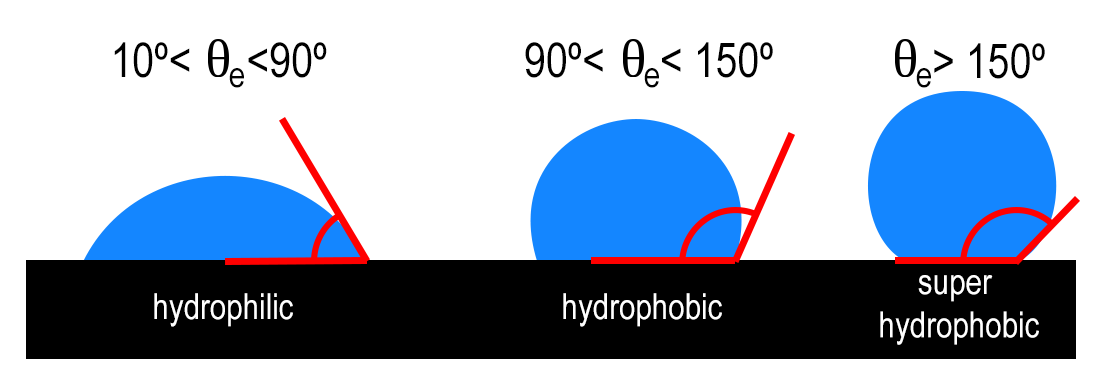
\includegraphics[width=0.7\linewidth]{Figures/2.Chapter/wet.png}
\caption{Wetting Regimes}
\label{fig:wet}
\end{figure}

\par Although it's been assumed that the surface is smooth, in reality one has to take in account the roughness of the surface. Considering an rough homogeneous interface, one can convert the smooth surface contact angle ($\theta_e$) to the actual contact angle ($\theta$) using a formula based on the force balance and empirical correlations, presented in Equation \ref{eq:wenzel}. 
\begin{equation}\label{eq:wenzel}
cos \theta = R_f cos \theta_e
\end{equation}
where $R_f= \frac{A_{SL}}{A_{F}}$ and is the relation between the surface area, to its flat projected area. This equation is called the Wenzel equation \cite{wenzel1936resistance}. Cassie took a different approach and considered an heterogeneous interface, where air would be trapped between the liquid and the surface, in the pockets formed by the surface roughness. So having an interface with a fraction $f_1$ at one contact angle $\theta_1$ and another at $f_2$ and $\theta_2$, the contact angle would be given by Cassie's Equation \cite{cassie1944wettability} :
\begin{equation}\label{eq:cassie}
cos \theta = f_1 cos \theta_1 + f_2 cos \theta_2
\end{equation}
\par The difference between both approaches can be seen in Figure \ref{fig:wenzelcassie}

\begin{figure}[h]
\centering
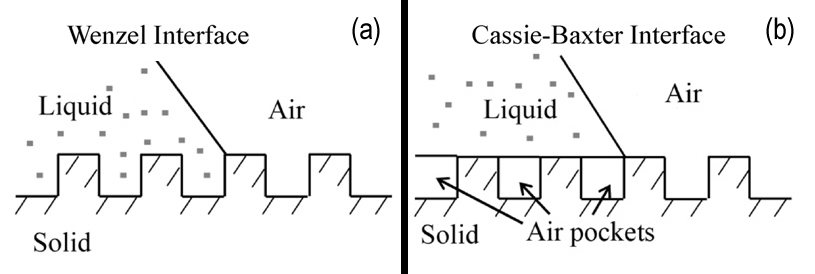
\includegraphics[width=0.7\linewidth]{Figures/2.Chapter/wenzelcassie.png}
\caption{Contact Angle approaches: (a) Wenzel, (b) Cassie-Baxter}
\source{Adapted from Bhushan, 2011\cite{bhushan2011natural}}
\label{fig:wenzelcassie}
\end{figure}


\section{Droplet Impact}

\par During droplet impacts it's possible to categorize the outcome in several categories :

\begin{itemize}
\item Rebound: after the impact the droplet leaves the surface partially or fully. Partial rebound happens when the surface is hydrophobic, and full rebound when it's super-hydrophobic.
\item Stick and Spread: the droplet sticks to the surface after the impact, spreading to its sides. This is characteristic of hydrophilic surfaces.
\item Splashing: the droplet sticks to the surface but smaller droplets are released in the spreading phase. This is influenced mainly by the impact speed and surface roughness.
\end{itemize}

\par When the droplet collides independently of the out come it deforms and spreads. The speed of the \textit{spreading} is dictated by the velocity of the contact edge ($u_{ce}$). This parameter relates with the droplet impact speed ($u_i$) and the contact angle ($\theta$) using Equation \ref{eq:droplet}.
\begin{equation} \label{eq:droplet}
u_{ce}=\frac{u_i}{tan \theta}
\end{equation}

\par During the impact another important parameter to analyze is the spreading factor $\beta$, described in Equation \ref{eq:beta}.
\begin{equation}\label{eq:beta}
\beta=D/d_0
\end{equation}

\par Finally it is possible to prove that the spreading factor grows with the impact velocity ($u_i$) and spreading time using Equation \ref{eq:rein}, taken from \cite{rein1993phenomena}:

\begin{equation}\label{eq:rein}
\beta(\tau)=1-exp(-c\tau) \text{, \quad where} \quad \tau=\frac{t u_i}{R}
\end{equation}

where c is a non-dimensional parameter that depends on the surface tension and R is the droplet radius at that time. This equation is only valid until it reaches the maximum spreading factor.

\par During the \textit{spreading}, when the diameter reaches its maximum value, the droplet assumes a shape similar to a disk. It is after that the \textit{recoiling} phase comes, decreasing the diameter. In this phase, wettability is very important, because it decides whether the droplet will stabilize or leave the surface. While the time-frame for the \textit{spreading} phase is short, the time-frame for the \textit{recoiling} is longer as the interactions between the droplet and the surface. In the final phase, for the hydrophilic surfaces, the droplet reaches an equilibrium diameter. The mentioned phenomena can be seen in Figure \ref{fig:droplet} and Figure \ref{fig:droplethf}.

\begin{figure}[h]
\centering
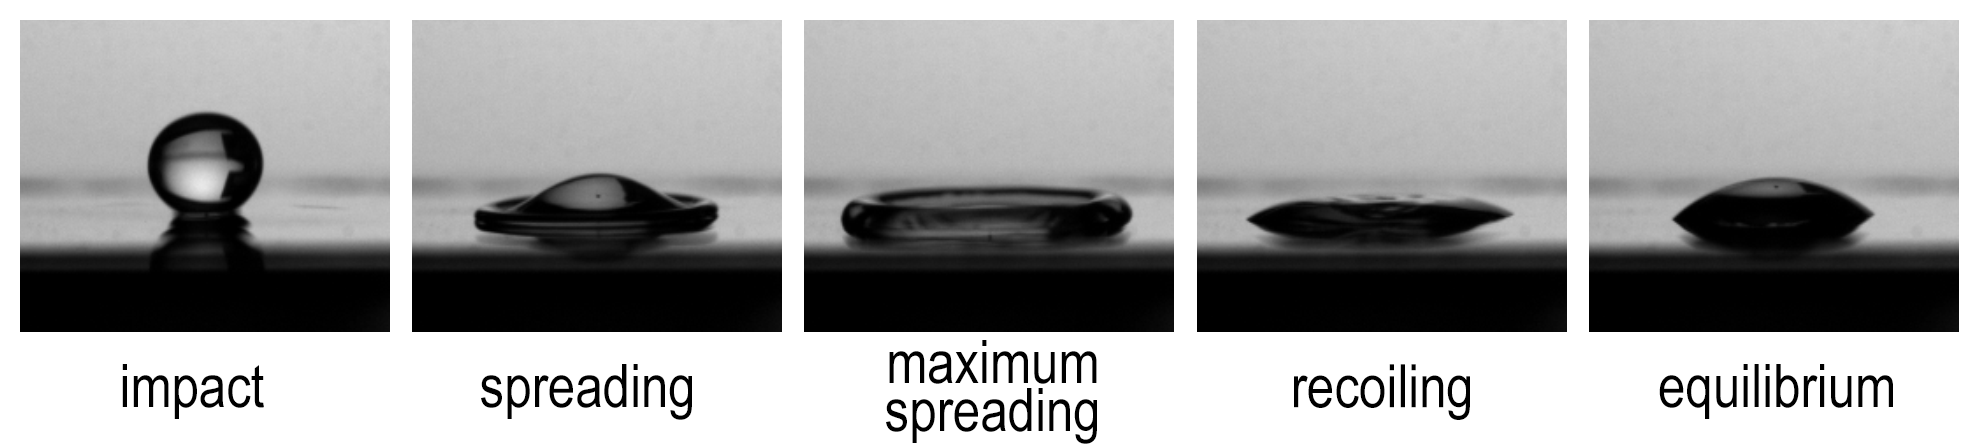
\includegraphics[width=0.9\linewidth]{Figures/2.Chapter/droplet.png}
\caption{Droplet impact stages, for an hydrophilic surface}
\label{fig:droplet}
\end{figure}

\begin{figure}[h]
\centering
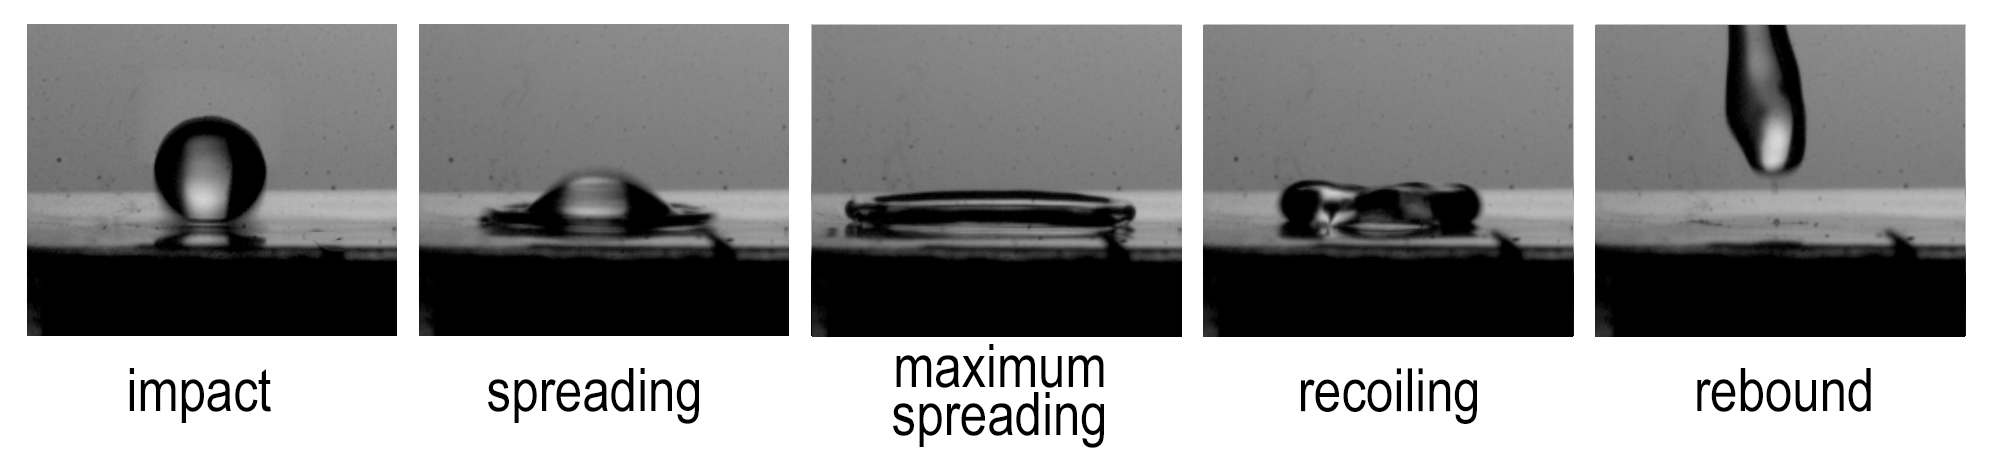
\includegraphics[width=0.9\linewidth]{Figures/2.Chapter/droplethf.png}
\caption{Droplet impact stages, for an hydrophobic surface}
\label{fig:droplethf}
\end{figure}

\par At higher speeds \textit{fingering} may happen. This happens due to instabilities at high Reynolds number that cause the spread droplet to loose its symmetry and form waves at the edge that are called \textit{fingers}. This phenomena can be seen in Figure \ref{fig:fingering}

\begin{figure}[h]
\centering
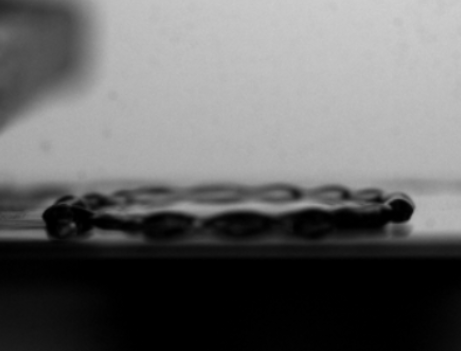
\includegraphics[width=0.35\linewidth]{Figures/2.Chapter/fingering.png}
\caption{Fingering}
\label{fig:fingering}
\end{figure}

\section{Heat Transfer}
\label{sec:heat}

\par During a droplet impact, the most important heat flux to evaluate is the change of heat between the droplet and the heater. According to \cite{sielaff2014experimental}, the heat flux from the droplet can be written as:

\begin{equation}
q''=q_0''+k_h \delta (\frac{{\partial}^2 T}{\partial x^2}+\frac{{\partial}^2 T}{\partial y^2})-\rho_h c_{p,h} \delta \frac{{\partial} T}{\partial t} \quad [W/m^2]
\end{equation}

were $q_0$ is the heat flux from the heater, $k_h$, $\rho_h$ and $c_{p,h}$ are the conductivity, density and specific heat capacity of the heater's material and $\delta$ is the thickness of the heater. Across the radius of the droplet, the heat flux can assume shape shown in Figure \ref{fig:fluxo}. High heat transfer is detected in the first moments before impact, and there is a peak near the edge of the droplet. This is the cause of "new" cold liquid reaching the hot surface. The heat flux is reduced substantially as time passes, mainly because the droplet is heating and the liquid speed is dropping, thus reducing convective and conductive heat transfer.

\begin{figure}[h]
\centering
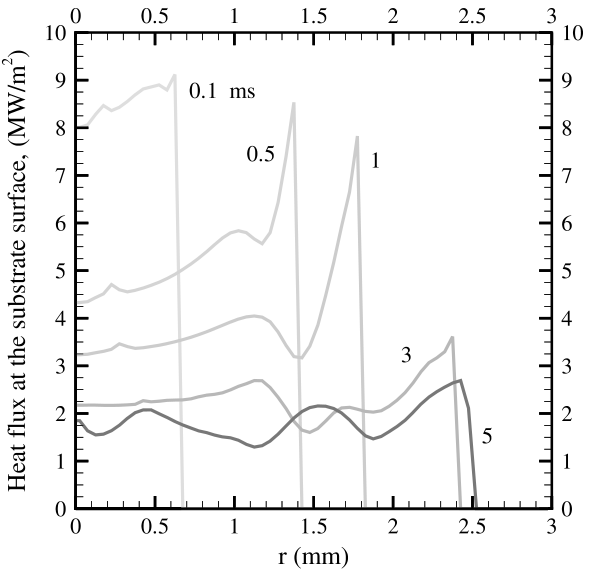
\includegraphics[width=0.5\linewidth]{Figures/2.Chapter/fluxo.png}
\caption {Heat Flux at the surface for different timesteps}
\label{fig:fluxo}
\source{M. Pasandideh-Fard, 2001 \cite{pasandideh2001cooling}}
\end{figure}

\par The power dissipated ($P_{diss}$) by the droplet is the integral of this expression in the droplet area, and it's given by:

\begin{equation}\label{eq:diss}
P_{diss}= \int_{A} q'' \; dA \quad [W]
\end{equation}

\par Because the droplet, ideally, is always axisymetric, it is necessary to decompose $dA$ in cylindrical coordinates. Equation \ref{eq:diss} is expressed in cylindrical coordinates in Equation \ref{eq:cyl}. Integrating the power in time we end up with the total heat extracted. This is expressed in Equation \ref{eq:qtot}.

\begin{equation} \label{eq:cyl}
P_{diss} = \int_\theta \int_r r \, q'' \; dr d\theta \quad [W]
\end{equation}
\begin{equation} \label{eq:qtot}
Q_{tot} = \int_t P_{diss} \; dt [J]
\end{equation}

\par In the work of Pasandideh-Fard \cite{pasandideh2001cooling} is proposed a way to quantify the "cooling effectiveness" ($\epsilon$) of the droplet. This effectiveness is described by the actual heat removed by the droplet divided by the maximum heat transfer possible by theory (assuming no phase change). This coefficient is described by Equation \ref{eq:epsilon}.\\

\begin{equation}\label{eq:epsilon}
\epsilon= \frac{\int_t \int_A q'' \; dA \, dt}{(m c_p \Delta T)_{water}}
\end{equation}

\par The relation between the cooling effectiveness and the time adimensionalized for different impact velocities has already been computed in the past \cite{pasandideh2001cooling} and is shown in Figure \ref{fig:cooling}. The cooling effectiveness grows with the impact velocity because, as shown in Equation \ref{eq:rein}, the spreading factor is larger, meaning that the area covered by the droplet also grows.

\begin{figure}[h]
\centering
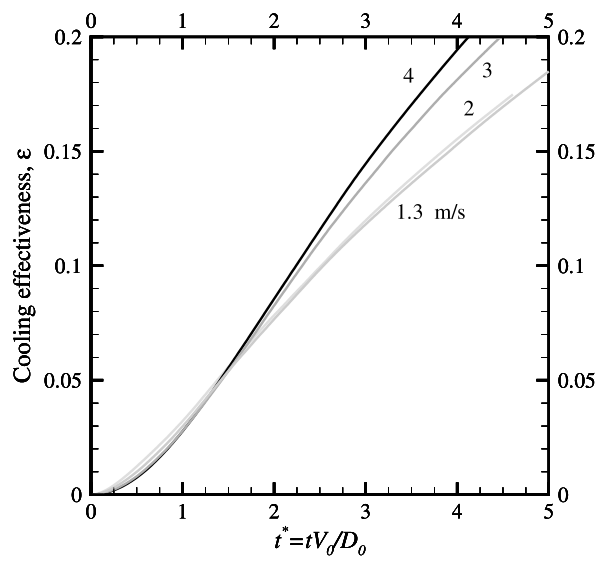
\includegraphics[width=0.5\linewidth]{Figures/2.Chapter/cooling.png}
\caption {Evolution of the calculated cooling effectiveness during the impact of a droplet on a surface initially at 120ºC}
\label{fig:cooling}
\source{M. Pasandideh-Fard, 2001 \cite{pasandideh2001cooling}}
\end{figure}

\par During droplet impact there are many phases that have special heat transfer characteristics. It is described in various sources (e.g. \cite{strotos2011non}) the variation of temperature in the droplet. The Figure \ref{fig:tempvar} illustrates approximately how the temperature of the surface evolves along the radius during spreading. In the center of the droplet the bubble trapping effect creates a barrier for heat transfer, this causes the temperature to have a slightly higher value. Also in the minimum thickness area, also called neck, in the literature, the temperature is higher because the layer of liquid is thinner, removing less heat. In the contact edge, liquid that accumulates there. This liquid comes from the center of the droplet and is colder then the liquid already there, so the temperature decreases again in the edge. The temperature then returns to the heater's temperature, a small distance after the contact edge due to heat conduction in the heater.

\begin{figure}[h]
\centering
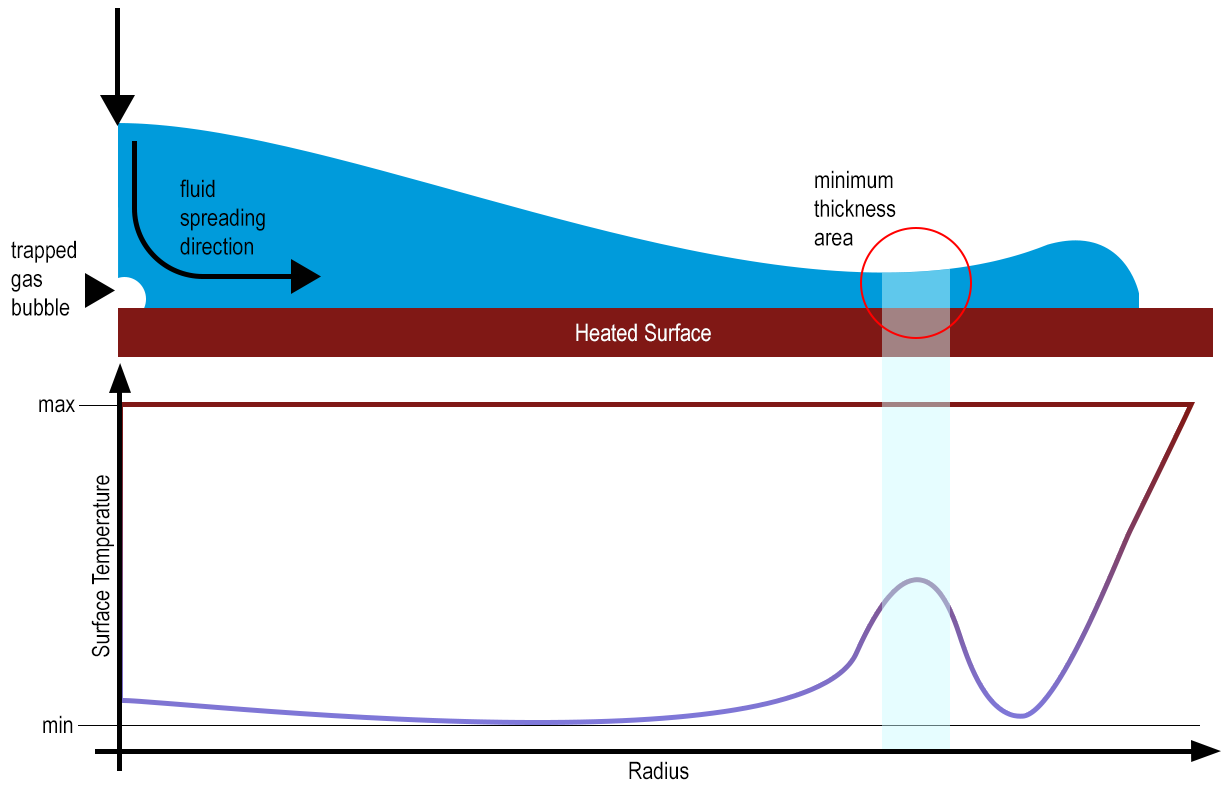
\includegraphics[width=1\linewidth]{Figures/2.Chapter/tempvar.png}
\caption {Scheme of the surface temperature variation along the droplet radius, during spreading}
\label{fig:tempvar}
\end{figure}



\cleardoublepage

% %%%%%%%%%%%%%%%%%%%%%%%%%%%%%%%%%%%%%%%%%%%%%%%%%%%%%%%%%%%%%%%%%%%%%%
% The Introduction:
% %%%%%%%%%%%%%%%%%%%%%%%%%%%%%%%%%%%%%%%%%%%%%%%%%%%%%%%%%%%%%%%%%%%%%%
\fancychapter{Conclusions and Future Work}
\label{cap:conclusions}

Conclusions Chapter

\cleardoublepage
\cleardoublepage
\phantomsection
\addcontentsline{toc}{chapter}{Bibliography}
\bibliographystyle{IEEEtran}
\bibliography{02.biblio}
\cleardoublepage

\begin{appendices}
	\begin{appendix}
		\pagenumbering{bychapter}
		\chapter{MATLAB function: calibration.mat}
\label{ap:a}
\lstset{
    frame=tb, % draw a frame at the top and bottom of the code block
    tabsize=4, % tab space width
    showstringspaces=false, % don't mark spaces in strings
    numbers=left, % display line numbers on the left
    commentstyle=\color{green}, % comment color
    keywordstyle=\color{blue}, % keyword color
    stringstyle=\color{red} % string color
}
\begin{lstlisting}[language=matlab]
function vid=calibration(vid)

L=size(vid); %extrai tamanho da matriz do video
x=600; %inicializacao do valor
Tamb=24; %temperatura ambiente
e=0.95; %emissividade estimada

for k=1:L(3)
    for j=1:L(2)
        for i=1:L(1)
            ADU = vid(i,j,k);
            %seguranca para excluir pixeis mortos
            if ADU < 1000
                vid(i,j,k) = 450;
            else
                %encontra Wtot para ADU de cada pixel
                r=roots([-1.4901E-6 8.4705E-3 -3.268533 1574.11-ADU]);
                l=1;
                %filtra solucoes
                while l<4
                    fi=r(l);
                    if fi >=300 && fi<=1500
                        x = fi;
                    end
                    l=l+1;
                end
            end
            vid(i,j,k)=(nthroot((x/5.67E-8-0.05*(Tamb+273)^4)/e,4)-273);
        end
    end
    k
end
\end{lstlisting}   
		\cleardoublepage
	\end{appendix}
\end{appendices}


\end{document}